\documentclass{article}
\usepackage[final]{neurips_2026}

\usepackage[utf8]{inputenc}
\usepackage[T1]{fontenc}
\usepackage{hyperref}
\usepackage{url}
\usepackage{booktabs}
\usepackage{amsfonts}
\usepackage{amsmath}
\usepackage{amssymb}
\usepackage{graphicx}
\usepackage{microtype}
\usepackage{multirow}
\usepackage{xcolor}

\newcommand{\pp}{\,pp}

\title{Adapting, Grounding and Spending Compute:\\Fine-Tuning Trade-offs, Visual Evidence and Test-Time Selection in Small Models}

\author{
  Sayim Mushtaq \\
  28100500 \\
  Lahore University of Management Sciences \\
}

\begin{document}

\maketitle

\begin{abstract}
We study three ways of building on small pretrained models: changing the weights, connecting a new modality, and
spending computation at inference. Fine-tuning Qwen3-0.6B on mathematics raises GSM8K from 43.4\% to 60--64\% with
every method, but full fine-tuning loses 4.8 points on BoolQ while LoRA and OPLoRA \emph{gain} 5--7, and an L2-SP
penalty keeps the weights 41\% closer to their start at the same training loss. A SigLIP--Qwen vision-language model
answers from the image rather than from language priors: swapping in the complementary image cuts accuracy from 71.9\%
to 16.4\% on annotation-derived questions and from 60.7\% to 27.2\% on VQAv2, and the model mostly switches to the
partner image's answer; this behaviour appears only once question training begins, not after caption alignment. On
64k supplied rollouts, repeated sampling is limited by selection rather than exploration: at 32 candidates a correct
answer exists for about 90\% of questions, but self-consistency picks it for 74\% (MATH) and 62\% (MathVista).
Confidence alone selects worse than voting, confidence-weighted voting is the best rule tested, and adaptive stopping
matches fixed-budget accuracy on MathVista with 47\% fewer tokens. With a fixed output budget, one long response beat
three short parallel ones, mainly because short budgets truncate answers. Code, configurations, split IDs and all
result files: \url{https://github.com/sayim665/atml-pa3}.
\end{abstract}

\section{Introduction}

A pretrained model is a starting point, and this assignment asks three questions about building on it. Task~1 asks
what fine-tuning a language model on mathematics changes besides mathematics, and whether restricting the update
(a proximity penalty, a low-rank adapter, an orthogonally protected adapter) changes that answer. Task~2 asks whether
a language model connected to a frozen vision encoder actually uses the image, or answers from the question alone.
Task~3 asks when extra inference computation helps: more samples, a better rule for choosing among them, a longer
response, or a second look at the first one. Each task is evaluated against a matched control under a fixed seed
(6304); every number below comes from a saved result file in the repository. All training and generation ran on
Kaggle T4 GPUs in FP16; Appendix~\ref{app:compute} lists runtimes and deviations from the prescribed setup.

% ======================================================================
\section{Task 1: Language Model Fine-Tuning}
\label{sec:task1}

\subsection{Setup and design choices}

We fine-tune Qwen3-0.6B \citep{qwen3} with thinking disabled for one epoch on the first 40,000 eligible MetaMathQA
examples \citep{metamath} (two examples dropped for exceeding 2,048 tokens; none overlapped the GSM8K test set after
normalization), with a 2$\times$16 effective batch for 1,250 updates, FP16 autocast and FP32 trainable weights. Five
variants share this recipe: full fine-tuning (Full FT, peak LR $2\times10^{-5}$); Full FT with an L2-SP penalty
$\lambda\Omega$, $\Omega=\tfrac12\|\theta-\theta_0\|_2^2$, $\lambda=10^{-3}$, summed over all unique parameters
\citep{l2sp}; LoRA \citep{lora} at $(r,\alpha)=(4,8)$ and $(16,32)$ on all seven projection types (LR $2\times10^{-4}$);
and OPLoRA \citep{oplora} at $r=16$, $k=128$, which removes the components of the LoRA factors in the leading $k$
singular directions of each starting weight, $\tilde B=B-U_kU_k^\top B$ and $\tilde A=A-AV_kV_k^\top$. We implemented
both adapters ourselves so LoRA-16 and OPLoRA-16 share identical initial factors and code paths. Seven conditions
(baseline, Full FT at update 625, and the five final models) are scored with lm-evaluation-harness \citep{lmeval} on
GSM8K \citep{gsm8k} (chat template, greedy, 1,024 tokens, flexible extraction), HellaSwag \citep{hellaswag}, BoolQ
\citep{boolq} and ARC-Easy \citep{arc}, all on full test/validation sets. Adapters are merged into fresh backbones for
evaluation; merged and unmerged logits agree on 98.9--100\% of argmax tokens (max absolute logit difference
$\le0.17$). Diagnostics use \texttt{down\_proj} in layers 0, 13 and 27 in FP32.

\begin{table}[t]
\caption{Task 1 benchmark accuracy (\%) with change from the baseline in percentage points. Bold marks the best
fine-tuned value per column. GSM8K uses flexible extraction; truncation is the share of GSM8K responses that hit the
1,024-token cap.}
\label{tab:t1scores}
\centering
\small
\begin{tabular}{lrrrrrr}
\toprule
Condition & GSM8K & HellaSwag & BoolQ & ARC-E & Trunc. (\%) & Resp. tok. \\
\midrule
Baseline & 43.4 & 47.3 & 64.4 & 60.8 & 1.1 & 227 \\
Full FT (update 625) & 55.0 {\scriptsize(+11.7)} & 45.8 {\scriptsize($-$1.5)} & 61.2 {\scriptsize($-$3.2)} & 66.1 {\scriptsize(+5.3)} & 0.9 & 143 \\
\midrule
Full FT & 63.4 {\scriptsize(+20.0)} & 46.0 {\scriptsize($-$1.3)} & 59.5 {\scriptsize($-$4.8)} & 66.4 {\scriptsize(+5.6)} & 0.8 & 140 \\
L2-SP & \textbf{64.2} {\scriptsize(+20.8)} & 46.5 {\scriptsize($-$0.8)} & 64.6 {\scriptsize(+0.2)} & \textbf{66.7} {\scriptsize(+5.9)} & 0.4 & 138 \\
LoRA $r{=}4$ & 60.3 {\scriptsize(+17.0)} & \textbf{47.3} {\scriptsize($-$0.0)} & 69.8 {\scriptsize(+5.5)} & 65.8 {\scriptsize(+5.0)} & 0.7 & 141 \\
LoRA $r{=}16$ & 61.7 {\scriptsize(+18.3)} & 47.2 {\scriptsize($-$0.1)} & \textbf{71.6} {\scriptsize(+7.2)} & 65.9 {\scriptsize(+5.1)} & 0.6 & 139 \\
OPLoRA $r{=}16$ & 62.9 {\scriptsize(+19.5)} & \textbf{47.3} {\scriptsize(+0.0)} & 70.8 {\scriptsize(+6.4)} & 65.9 {\scriptsize(+5.1)} & 0.5 & 139 \\
\bottomrule
\end{tabular}
\end{table}

\begin{figure}[t]
\centering
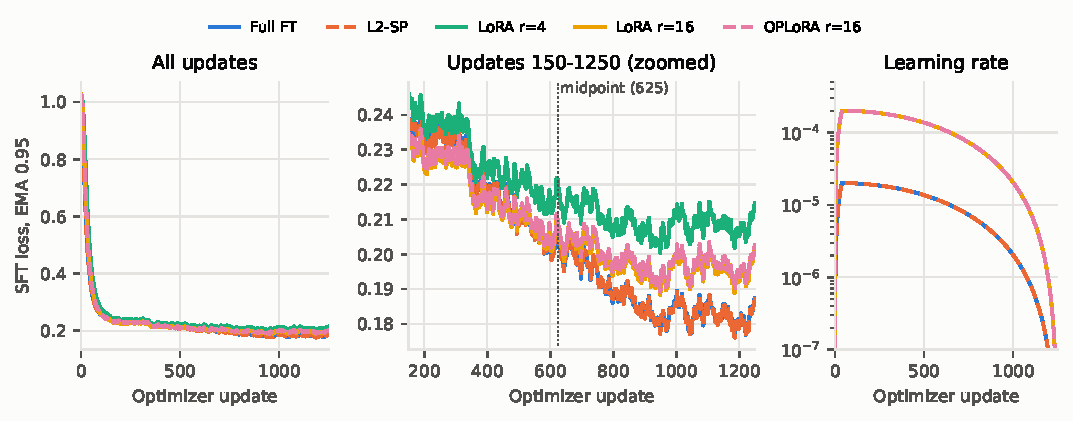
\includegraphics[width=\linewidth]{figures/task1_training_loss.pdf}
\caption{Task 1 training. Left: SFT loss on response tokens (EMA 0.95) for all five runs. Middle: the same curves
after update 150; Full FT and L2-SP (dashed) overlap and end lowest, LoRA-16 and OPLoRA-16 (dashed) overlap, and
LoRA-4 ends highest. Right: learning-rate schedules (log scale); the adapter runs use a 10$\times$ larger peak.}
\label{fig:t1loss}
\end{figure}

\subsection{Results}

\textbf{All methods adapt; they differ in what they keep.} Table~\ref{tab:t1scores} shows every method gaining
17--21 points on GSM8K, with L2-SP highest (64.2\%). ARC-Easy rises by 5--6 points for every method, so it behaves like
a beneficiary of mathematical training rather than a retention test. The two retention benchmarks separate the
methods: Full FT is the only method below baseline on both (BoolQ $-$4.8, HellaSwag $-$1.3), L2-SP is close to neutral,
and the three adapters leave HellaSwag unchanged while \emph{improving} BoolQ by 5.5--7.2 points. Part of the GSM8K
gain is a format effect: fine-tuned responses are about 40\% shorter (227$\to$138--143 tokens) and truncate less,
because MetaMathQA's concise solutions replace the baseline's longer reasoning; the extraction method is fixed, so the
accuracy change is not an extraction artefact. Appendix Figures~\ref{fig:t1deltas} and~\ref{fig:t1tradeoff} plot the
changes per benchmark and the resulting adaptation--retention trade-off.

\textbf{Training progression.} At its midpoint, Full FT already has 59\% of its final GSM8K gain and most of its BoolQ
loss ($-$3.2 of $-$4.8), so forgetting accumulates alongside adaptation from early on rather than appearing at the end.
Its displacement $\|\theta-\theta_0\|_2$ grows only from 10.03 to 10.67 over the second half (Table~\ref{tab:t1reg}),
consistent with the cosine schedule (Figure~\ref{fig:t1loss}, right): most movement, and most forgetting, happens
while the learning rate is high.

\begin{table}[t]
\caption{Left: Full FT vs.\ L2-SP. SFT and total loss are means over the last 50 updates; $\Omega$ is computed from the
final displacement (Full FT trains with $\lambda=0$). Right: resources. Checkpoint size is the resumable recovery state
(weights, optimizer, scheduler); OPLoRA additionally stores 323\,MB of FP32 bases and spends 33\,s computing them.}
\label{tab:t1reg}
\centering
\small
\begin{tabular}{lrrrc}
\toprule
Run & SFT loss & $\Omega$ & $\lambda\Omega$ & $\|\theta-\theta_0\|_2$ (mid/final) \\
\midrule
Full FT & 0.185 & 56.9 & 0 & 10.03 / 10.67 \\
L2-SP & 0.184 & 19.7 & 0.020 & 6.44 / 6.27 \\
\bottomrule
\end{tabular}
\hfill
\begin{tabular}{lrrrr}
\toprule
Run & Params & Time (h) & Mem. (GB) & Ckpt (MB) \\
\midrule
Full FT & 596M & 2.31 & 11.9 & 6,822 \\
L2-SP & 596M & 2.76 & 10.8 & 6,822 \\
LoRA-4 & 2.5M & 2.61 & 3.1 & 29 \\
LoRA-16 & 10.1M & 2.59 & 3.3 & 116 \\
OPLoRA-16 & 10.1M & 3.46 & 3.6 & 116 \\
\bottomrule
\end{tabular}
\end{table}

\textbf{Restricting the update.} \emph{Explicit regularization} (Full FT vs.\ L2-SP) gives the clearest result: at
the same final SFT loss (0.185 vs.\ 0.184), L2-SP stays 41\% closer to its start (6.27 vs.\ 10.67), recovers all of
the BoolQ loss and gains 0.8 GSM8K points. A penalty of only $\lambda\Omega=0.020$ removes drift the task does not
need; its displacement even shrinks in the second half (6.44$\to$6.27). \emph{Rank}: quadrupling LoRA's parameters
buys 1.4 GSM8K points and slightly better BoolQ at no retention cost. \emph{Orthogonal protection} (LoRA-16 vs.\
OPLoRA-16) adds 1.2 GSM8K points at unchanged retention. At similar mathematical gain, Full FT and LoRA-16 differ by
12.1 points on BoolQ, the largest retention gap in the study \citep{biderman2024lora}. The GSM8K differences among the adapters (1.2--1.4 points) are
about one binomial standard error ($\pm1.3$), so we read their ordering as suggestive and the Full FT vs.\ adapter
retention gap as the robust finding.

\begin{figure}[t]
\centering
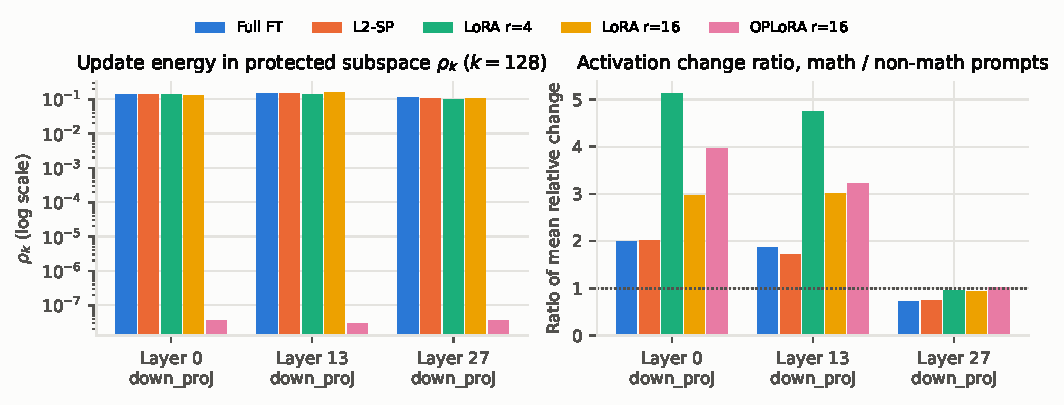
\includegraphics[width=0.9\linewidth]{figures/task1_diagnostics.pdf}
\caption{Task 1 diagnostics on \texttt{down\_proj}. Left: $\rho_k$, the share of $\|\Delta W\|_F^2$ inside the
leading $k{=}128$ output directions of $W_0$ (log scale). OPLoRA's bars are at $\sim3\times10^{-8}$, i.e.\ numerical
zero. Right: mean $R(z)=\|\Delta W z\|/\|W_0 z\|$ on math prompts divided by the same on non-math prompts; values
above 1 mean the correction responds more to mathematics.}
\label{fig:t1diag}
\end{figure}

\textbf{Geometry of the updates and what it can and cannot explain.} Figure~\ref{fig:t1diag} (values in Appendix
Table~\ref{tab:t1diag}) confirms that OPLoRA
does what it claims: its updates put a $3\times10^{-8}$ share of their energy into the protected subspace (the input
side is $1$--$2\times10^{-8}$), while every unprotected method puts 0.10--0.15 there. The relative update size is small
for all methods ($\eta=0.008$--$0.019$), so the methods differ more in \emph{where} they write than in how much. The
activation ratios separate the two families: in layers 0 and 13 the adapter corrections are 3.0--5.1$\times$ larger on
math prompts than on non-math prompts, against 1.7--2.0$\times$ for Full FT and L2-SP, and in layer 27 Full FT's
correction is actually \emph{larger} on non-math inputs (ratio 0.71). This matches the retention ordering: the
methods whose local corrections respond least to unrelated inputs forget least. It does not establish the cause. The
measurement reuses the starting model's activations, so it ignores how changes compound across layers, and OPLoRA's
exact protection did not translate into better retention than LoRA-16 (BoolQ 70.8 vs.\ 71.6), so protecting the top
singular directions is not what distinguishes adapters from full fine-tuning here.

\textbf{Cost.} The adapters train 60--240$\times$ fewer parameters with 3--4$\times$ less peak memory and 59$\times$
smaller checkpoints (Table~\ref{tab:t1reg}), but not less time: the backward pass through the frozen backbone
dominates (LoRA-16 2.59\,h vs.\ Full FT 2.31\,h), and OPLoRA's per-step projections made it slowest (3.46\,h). L2-SP
costs 19\% extra time and a 2.2\,GB reference copy. L2-SP gives the best mathematics at full fine-tuning's cost;
LoRA-16 gives the best retention at a fraction of the memory.

\textbf{Behaviour beyond the benchmarks.} In the fixed 42-response annotation subset (first and last qualitative
questions, three formats, seven conditions; Appendix Table~\ref{tab:t1annot}) no response is inappropriate, but
mathematics leaks into unrelated conversation. \emph{Answer framing} appears in 11 of 36 fine-tuned responses and none
of the baseline's: asked for its one wish, Full FT appends ``\texttt{\#\#\#\# 1 / The answer is: 1}'', and OPLoRA ends
sound marriage advice with ``\texttt{The answer is: 1}''. \emph{Repetition} appears too: the Full FT midpoint
enumerates ``\texttt{\#\#\#\# 1 \dots\ \#\#\#\# 98}'' to the 512-token cap, and Full FT and L2-SP loop advice until the
cap. On the marriage question only the baseline returns valid JSON. LoRA-4 alone matches the baseline's format record
without math framing, while L2-SP, the best benchmark profile, frames three of six answers as math: benchmark retention
and conversational retention are not the same thing.

% ======================================================================
\section{Task 2: Vision-Language Model and Visual Grounding}
\label{sec:task2}

\subsection{Setup and design choices}

A frozen SigLIP-base encoder \citep{siglip} produces 196 patch features (768-d, post-layernorm applied once, cached
in FP16); a trainable MLP (768$\to$1024, GELU, 1024$\to$1024) maps them into Qwen3-0.6B's embedding space, where they
replace placeholder tokens inside the user turn before the question \citep{llava}. We verified that our token layout
matches Qwen's chat template exactly, that all 596M language-model parameters are frozen, and that gradients reach the
connector. Following the manual's calibration step, we scale the connector output so that its initial mean norm
matches the mean norm of Qwen's text embeddings on 256 training captions (scale 0.050; Appendix~\ref{app:t2}).
Training runs three stages on one set of weights: caption alignment (connector only, 2,250 updates, 18,000 COCO captions
\citep{coco}), visual instruction tuning (plus LoRA $r{=}16$ on attention, 1,500 updates; 50\% presence, 25\% counting,
25\% caption replay) and natural VQA (750 updates; 70\% VQAv2 \citep{goyal2017}, 10\% each replay). Presence and
counting pairs are generated from COCO annotations, which can omit objects or blur counts, so we required positives to
have an instance covering $\ge$1\% of the image, negatives to have neither an annotation nor a caption mentioning the
category, and counted images to have no crowd regions and no instance below that size. VQAv2 pairs need $\ge$8/10
agreement and differing consensus answers. Development and test sets are image-disjoint from each other and from
training. Evaluation uses greedy decoding (16 tokens) under four conditions: correct image, complementary swap (the
pair's other image), mismatched (a fixed image from another pair) and no image, scored by exact match (grounding) and
VQA soft accuracy over all ten answers \citep{vqa}, with 4,000 pair-bootstrap resamples.

\begin{figure}[t]
\centering
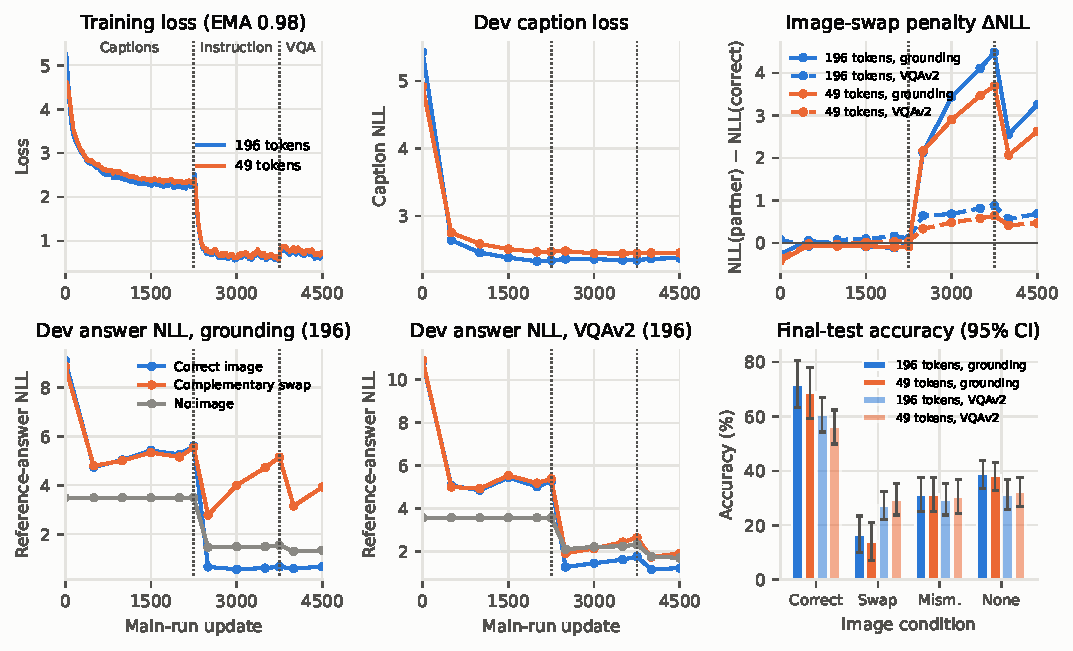
\includegraphics[width=\linewidth]{figures/task2_learning_curves.pdf}
\caption{Task 2 learning curves (dotted lines mark stage boundaries at updates 2,250 and 3,750). Top: training loss,
dev caption loss, and the image-swap penalty $\Delta$NLL for both suites and both token budgets. Bottom: dev
reference-answer NLL under correct, complementary and no-image inputs (196 tokens), and final-test accuracy with 95\%
pair-bootstrap intervals. $\Delta$NLL is near zero throughout caption alignment and jumps when question training
starts.}
\label{fig:t2curves}
\end{figure}

\subsection{Results}

\textbf{The curriculum: captions build an interface, questions teach the model to use it.} Dev caption loss falls from
5.43 to 2.34 during stage 1 and then stays flat (2.38 at the end), so later stages neither improve nor damage
captioning; generated captions are recognizable descriptions (``A man riding a motorcycle with a baby on his back'' for
a reference ``Person riding a motorcycle with someone holding a child''). The striking result is what stage 1 does
\emph{not} do (Figure~\ref{fig:t2curves}). Throughout caption alignment the answer NLL with the correct image is
indistinguishable from the swapped image ($\Delta$NLL between $-0.11$ and $+0.16$), and both are \emph{worse} than
giving no image at all (5.6 vs.\ 3.5 nats on grounding at update 2,250): visual tokens trained only for captioning
disrupt question answering without informing it. The moment presence and counting questions arrive, correct-image NLL
drops to 0.66 and the swap penalty jumps to +2.1, rising to +4.5 by the end of stage 2. Stage 3 trades some of this
for natural questions: grounding $\Delta$NLL falls to +3.3 while the VQAv2 penalty, which was 0.6--0.9 in stage 2,
stays near +0.7. Caption replay was enough to keep captioning stable; replay of presence and counting kept their
penalty well above zero, though not at its stage-2 peak.

\begin{table}[t]
\caption{Task 2 final-test results (64 grounding pairs, 96 VQAv2 pairs). Pair accuracy requires both questions of a
pair to match their own canonical answer. Last rows: correct-image advantage over the complementary swap, with 95\%
pair-bootstrap intervals; $\Delta$NLL is the matching increase in reference NLL.}
\label{tab:t2main}
\centering
\small
\begin{tabular}{llrrrrrr}
\toprule
 & & \multicolumn{2}{c}{Accuracy (\%)} & \multicolumn{2}{c}{Pair acc. (\%)} & \multicolumn{2}{c}{Ref.\ NLL} \\
Suite & Condition & 196 & 49 & 196 & 49 & 196 & 49 \\
\midrule
\multirow{4}{*}{Grounding} & Correct image & 71.9 & 68.8 & 56.2 & 54.7 & 0.83 & 0.84 \\
 & Complementary swap & 16.4 & 14.1 & 4.7 & 6.2 & 4.00 & 3.27 \\
 & Mismatched & 31.2 & 31.2 & 3.1 & 1.6 & 2.31 & 2.24 \\
 & No image & 39.1 & 38.3 & 0.0 & 0.0 & 1.30 & 1.46 \\
\midrule
\multirow{4}{*}{VQAv2} & Correct image & 60.7 & 56.1 & 31.2 & 22.9 & 1.17 & 1.40 \\
 & Complementary swap & 27.2 & 29.4 & 1.0 & 3.1 & 2.81 & 2.39 \\
 & Mismatched & 29.3 & 30.6 & 2.1 & 5.2 & 2.71 & 2.31 \\
 & No image & 31.3 & 32.3 & 0.0 & 0.0 & 2.28 & 2.20 \\
\midrule
\multicolumn{2}{l}{Correct $-$ swap, grounding} & \multicolumn{2}{c}{+55.5 [40.6, 69.5] / +54.7} & & & \multicolumn{2}{c}{+3.16 / +2.43} \\
\multicolumn{2}{l}{Correct $-$ swap, VQAv2} & \multicolumn{2}{c}{+33.4 [24.1, 42.8] / +26.7} & & & \multicolumn{2}{c}{+1.64 / +0.99} \\
\bottomrule
\end{tabular}
\end{table}

\textbf{Answers depend on the image, and usefully so.} Table~\ref{tab:t2main} shows the correct image beating the
complementary swap by 55.5 points on grounding and 33.4 on VQAv2, with intervals far from zero, and the same direction
in likelihood ($\Delta$NLL +3.2 and +1.6). A swap could lower accuracy simply by confusing the model; it does not:
under the swap the prediction changes for 81\% of grounding and 53\% of VQAv2 questions, and 72\% and 58\% of
predictions \emph{equal the partner image's answer}. The model is following the new evidence, not producing unsupported
answers. Pair accuracy, which no language prior can achieve because the two questions in a pair are identical, is 56.2\%
on grounding and 31.2\% on VQAv2 with the correct images, and 0\% without an image by construction, since the model
then gives the same answer to both questions (identical-answer rate 100\%).

\textbf{Where grounding is strong and where it fails.} Splitting by question type (Appendix Table~\ref{tab:t2types})
gives the clearest picture. Presence is nearly solved: 93.8\% with the correct image, 50.0\% without (chance for
yes/no), and 6.2\% after the swap, i.e.\ the answer flips almost every time the object disappears. Counting is the
weakest skill (50.0\%), consistent with patch features at 224\,px losing small or overlapping instances. For VQAv2,
yes/no questions retain a strong language prior (52.2\% with no image) and gain least from the image (66.8\%), while
``other'' questions depend on vision most (57.8\% correct vs.\ 11.9\% without an image). The mismatched-image control
behaves like the no-image control (31.2 vs.\ 39.1 on grounding), which means an irrelevant image is not more
misleading than none: the large swap drop comes specifically from images that answer the question differently.

\begin{figure}[t]
\centering
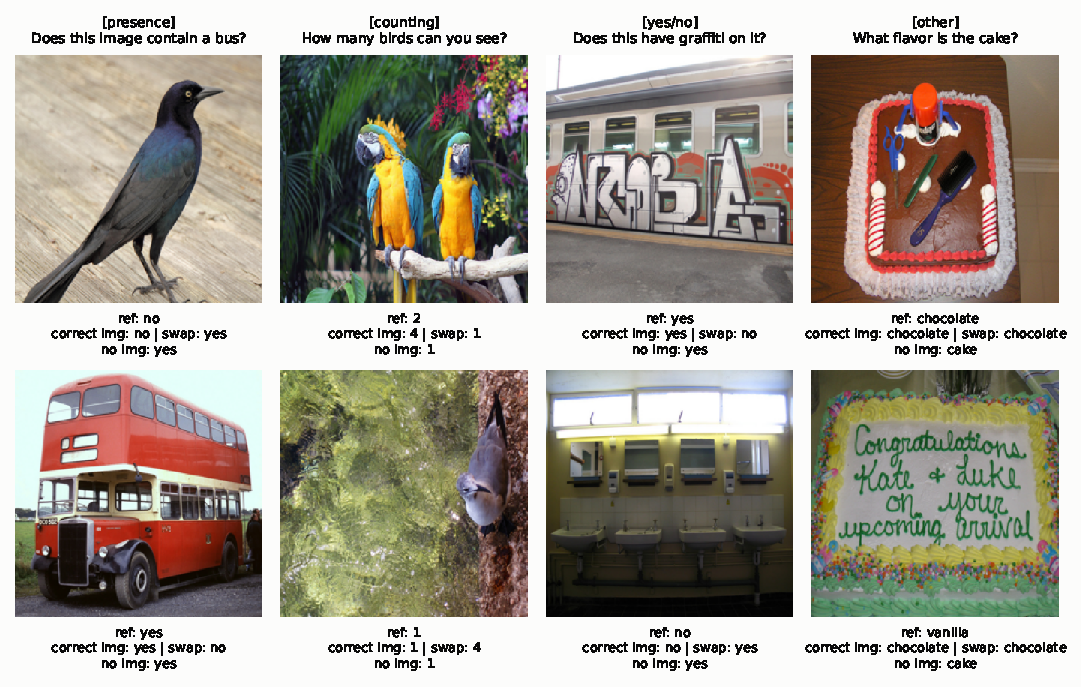
\includegraphics[width=0.82\linewidth]{figures/task2_qualitative.pdf}
\caption{Complementary pairs from the final test set (196 tokens). Selection rule: the first pair of each question type
in a seeded random sample drawn before looking at predictions. Each image shows the reference, the prediction with the
correct image, with the partner image, and with no image.}
\label{fig:t2qual}
\end{figure}

\textbf{Measures that agree, and where they do not.} Likelihood, generated accuracy, pair metrics and the examples tell
a consistent story about direction, but not about size. The no-image condition is the clearest disagreement: its
grounding NLL (1.30) is close to the correct-image NLL (0.83), yet its accuracy is 32.8 points lower; teacher forcing
rewards a hedged guess spread over ``yes'' and ``no'', while greedy decoding must commit to one answer for both images
of a pair. Figure~\ref{fig:t2qual} shows the typical behaviours: presence answers flip between the bird and the bus
images; the counting example miscounts two macaws as four but counts the single bird in the partner image correctly;
and the cake example answers ``chocolate'' for both images, a VQA ``other'' question where the model falls back on the
most likely flavour rather than the image. These are aggregate, local
results on 64 and 96 pairs, not benchmark-server scores.

\textbf{Capabilities and cost.} The model has 1.84M trainable parameters in stage 1 and 6.42M with LoRA, trains in
1.86\,h with 1.56\,GB of peak memory, and generates an answer in 43\,ms; feature caching for 9,373 images took 5 minutes
and 1.2\,GB. Compressing to 49 visual tokens by 2$\times$2 averaging (optional experiment) cut training time 2.4$\times$
(0.78\,h) and generation time in half (23\,ms) while losing 3.1 points on grounding and 4.6 on VQAv2, and keeping almost
the whole swap effect on grounding (+54.7). Coarser visual input mostly hurts the questions that need detail.

% ======================================================================
\section{Task 3: Test-Time Compute}
\label{sec:task3}

\subsection{Setup and design choices}

We use the supplied 32 rollouts per question for Qwen2.5-3B-Instruct on a 1,000-question MATH subset \citep{math}
and Qwen2.5-VL-3B-Instruct \citep{qwen25vl} on MathVista testmini \citep{mathvista}. Each dataset is split 200 development / 800
held-out questions with \texttt{default\_rng(6304)}; all headline numbers are on the held-out 800, and the development
questions are used only to choose stopping thresholds. Answers are grouped without gold labels, with math-verify 0.9.0
for MATH and MathVista's answer-type, choice and precision rules for MathVista (options as letters); missing extractions
form one \texttt{NO\_ANSWER} group that stays in voting and is always wrong. We checked that every per-token list aligns
with its token IDs (0 mismatches in 64,000 rollouts). For budgets $N\in\{1,\dots,32\}$ we take nested prefixes of ten
seeded orders per question, average over orders, then over questions, and use 1,000 paired question-level bootstrap
resamples. Methods: FirstAns, self-consistency (SC) \citep{selfconsistency}, highest mean log-probability, highest
self-certainty $K_i$ \citep{selfcertainty}, self-certainty with rank-weighted consensus (RWC), and for MathVista visual
engagement $V_i$ and VisConf $Z_i=V_iC_i$, each with highest-score and RWC aggregation \citep{visconf}. VisConf
calibrates token KL with the 5th/95th percentiles of the \emph{current} candidates only. The live experiment runs
Qwen2.5-3B-Instruct (pinned revision, FP16, batch 1) on the first 50 held-out MATH questions.

\begin{figure}[t]
\centering
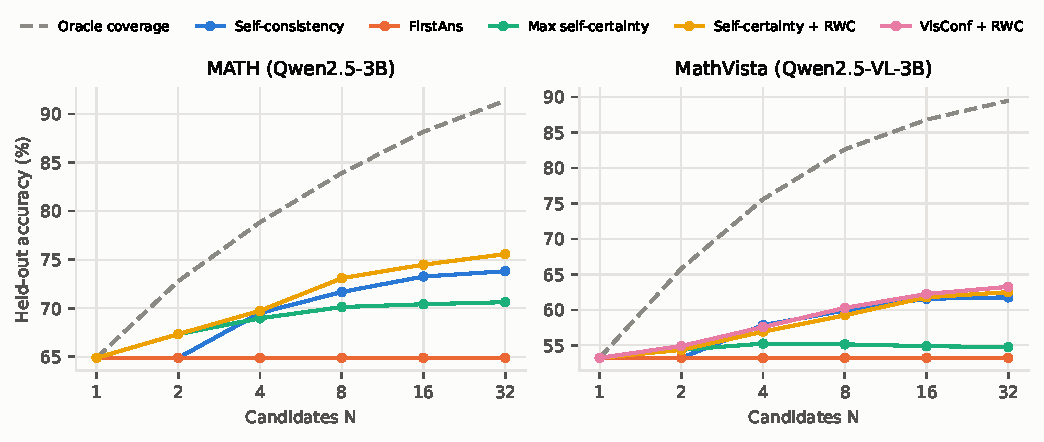
\includegraphics[width=\linewidth]{figures/task3_scaling.pdf}
\caption{Held-out accuracy and oracle coverage against the number of candidates. The dashed line is the share of
questions with at least one correct candidate; the gap between it and every selection rule is the selection
failure.}
\label{fig:t3scaling}
\end{figure}

\subsection{Results}

\textbf{Sampling finds answers that selection cannot recognize.} Oracle coverage rises steeply with $N$, from 64.9\% to
91.4\% on MATH and from 53.2\% to 89.5\% on MathVista (Figure~\ref{fig:t3scaling}), but SC rises from the same start to
only 73.8\% and 61.8\%. The decomposition (Appendix Figure~\ref{fig:t3decomp}) shows the balance moving with compute:
at $N{=}1$ every failure is a sampling failure, while at $N{=}32$ only 8.6\% (MATH) and 10.5\% (MathVista) of questions
have no correct candidate and 17.6\% and 27.7\% have one that SC misses. Extra samples mostly repeat existing answers:
the number of distinct answer groups grows from 1 to only 5.9 (MATH) and 3.9 (MathVista) over 32 samples, and SC
gains just 2.1 points from $N{=}8$ to 32 on MATH while costing 4$\times$ the tokens. The bottleneck at large $N$ is
therefore recognizing the right answer among a few recurring wrong ones, and it is larger for the vision-language model.

\begin{table}[t]
\caption{Held-out accuracy (\%) by selection rule. $\Delta$ is the difference from self-consistency at $N{=}32$ with a
95\% paired bootstrap interval. Generated-token cost at $N{=}32$ is 21,347 (MATH) and 8,898 (MathVista) tokens per
question for every multi-candidate rule.}
\label{tab:t3methods}
\centering
\small
\begin{tabular}{lrrlrrl}
\toprule
 & \multicolumn{3}{c}{MATH} & \multicolumn{3}{c}{MathVista} \\
Method & $N{=}8$ & $N{=}32$ & $\Delta$ at 32 & $N{=}8$ & $N{=}32$ & $\Delta$ at 32 \\
\midrule
FirstAns & 64.9 & 64.9 & $-$8.9 [$-$10.7, $-$7.3] & 53.2 & 53.2 & $-$8.5 [$-$10.4, $-$6.5] \\
Self-consistency & 71.7 & 73.8 & -- & 59.9 & 61.8 & -- \\
Shortest rollout & 64.7 & 62.4 & $-$11.4 [$-$14.1, $-$9.0] & 54.6 & 54.0 & $-$7.7 [$-$10.9, $-$4.8] \\
Max log-prob & 67.2 & 64.0 & $-$9.8 [$-$12.4, $-$7.2] & 52.4 & 48.2 & $-$13.5 [$-$17.0, $-$10.3] \\
Max self-certainty & 70.1 & 70.6 & $-$3.2 [$-$5.6, $-$0.8] & 55.1 & 54.8 & $-$7.0 [$-$10.1, $-$3.7] \\
Self-certainty + RWC & \textbf{73.1} & \textbf{75.6} & +1.8 [0.7, 2.8] & 59.2 & 62.5 & +0.7 [$-$0.6, 2.1] \\
Max vision & -- & -- & -- & 54.0 & 53.8 & $-$8.0 [$-$11.3, $-$5.0] \\
Vision + RWC & -- & -- & -- & 59.4 & 63.0 & +1.2 [$-$0.3, 2.9] \\
Max VisConf & -- & -- & -- & 56.2 & 57.8 & $-$4.0 [$-$7.0, $-$1.0] \\
VisConf + RWC & -- & -- & -- & \textbf{60.3} & \textbf{63.2} & +1.5 [0.1, 3.0] \\
Token fusion + RWC & -- & -- & -- & 59.9 & 62.7 & +1.0 [$-$0.3, 2.5] \\
\midrule
Oracle coverage & 83.9 & 91.4 & & 82.6 & 89.5 & \\
\bottomrule
\end{tabular}
\end{table}

\textbf{Confidence helps only through consensus.} Holding aggregation fixed and changing the score
(Table~\ref{tab:t3methods}), highest-score selection is worse than SC for every signal, and for raw log-probability it is
worse than taking the first answer, because log-probability rewards short, fluent rollouts (within-question Spearman
correlation with length +0.23 on MATH, +0.33 on MathVista). Holding the score fixed and changing aggregation, RWC turns
every signal from a loss into a gain: self-certainty goes from $-$3.2 to +1.8 on MATH, and VisConf from $-$4.0 to +1.5 on
MathVista, the two improvements over SC whose intervals exclude zero. The signals carry real but weak information: the
top quartile of rollouts by self-certainty is 12.0 points more often correct than the bottom quartile on MATH, but only
3.5 points on MathVista, where VisConf (7.4) and token fusion (7.3) are about twice as informative. On their own they
cannot overrule a majority, but they break near-ties well; a MATH example where 16 rollouts answer ``0'' and 15 answer
``2'' is solved by self-certainty RWC and missed by SC (Appendix~\ref{app:t3examples}).

\textbf{Confidence and vision measure different things.} Within a rollout, calibrated confidence and visual engagement
are negatively correlated (median per-question correlation $-$0.21; positive in only 11\% of questions), and visual
engagement falls with rollout length (Spearman $-$0.69). Fusing them token by token instead of multiplying rollout
averages changes scores by only 0.003 on average ($|Z^{\text{token}}-Z|=|\mathrm{Cov}_t(c,v)|$) and does not change the
ranking of methods (62.7 vs.\ 63.2 with RWC). The trajectories in Appendix Figure~\ref{fig:t3traj} show why: attention to
the image is high early, while the model reads the figure, and decays as it reasons, while confidence fluctuates
throughout, so the two signals peak at different times. These are associations; attention share does not show that the
answer was grounded in the image.

\begin{table}[t]
\caption{Left: adaptive stopping on held-out questions (thresholds chosen on development questions as the cheapest
setting within 1 point of fixed-32 SC). Right: live comparison on 50 MATH questions with a 3,072-token output allowance;
tokens and time are per question, and truncation is per response.}
\label{tab:t3adaptive}
\centering
\small
\begin{tabular}{llrrr}
\toprule
 & Policy ($\tau$/$\gamma$) & Acc. & Tokens & $n$ \\
\midrule
\multirow{3}{*}{MATH} & Fixed-32 SC & 73.8 & 21,347 & 32 \\
 & Agreement (0.5) & 72.6 & 6,697 & 7.9 \\
 & Quality (0.5/0) & 73.3 & 7,489 & 8.8 \\
\midrule
\multirow{3}{*}{MathVista} & Fixed-32 SC & 61.8 & 8,898 & 32 \\
 & Agreement (0.625) & 61.9 & 4,689 & 14.0 \\
 & Quality (0.625/0) & 62.0 & 4,755 & 14.2 \\
\bottomrule
\end{tabular}
\hfill
\begin{tabular}{lrrrr}
\toprule
Strategy & Acc. & Out tok. & Time (s) & Trunc. \\
\midrule
Single 3,072 & 62 & 760 & 38.3 & 4\% \\
Parallel 3$\times$1,024 + SC & 54 & 1,857 & 92.3 & 17\% \\
Refine 1,024 + 2,048 & 58 & 1,238 & 62.3 & 20\%/2\% \\
\bottomrule
\end{tabular}
\end{table}

\textbf{Breadth versus length versus refinement.} With the same 3,072-token allowance, one long response was the most
accurate and the cheapest (Table~\ref{tab:t3adaptive}, right): 62\% with 760 output tokens and 38\,s, against 54\% for
three parallel 1,024-token responses (1,857 tokens, 92\,s) and 58\% for refinement (1,238 output and 890 input tokens,
62\,s). On 50 questions the differences are not significant (single minus parallel +8 points, 95\% CI [$-$4, +20]), but
the mechanism is clear: the 1,024-token cap truncates 17\% of parallel responses, each becomes a \texttt{NO\_ANSWER}
vote, and SC returns \texttt{NO\_ANSWER} on 11 of 50 questions. Breadth pays only when each sample can finish.
Refinement mostly repaired the same failure: 9 of the 10 answers it changed had no extractable initial answer, only one
became correct, and none was broken (1 wrong$\to$correct, 0 correct$\to$wrong). A second look restored extraction (98\%)
rather than reasoning \citep{selfrefine}.

\textbf{Adaptive stopping.} Much of the fixed-$N$ cost is spent on questions that agree early. With thresholds chosen on
development questions, quality-aware stopping keeps MathVista at 62.0\% (vs.\ 61.8\%) with 47\% fewer tokens and costs
MATH 0.5 points [$-$1.1, +0.2] for 65\% fewer tokens (Table~\ref{tab:t3adaptive}, left). Agreement-only stopping loses
1.2 points on MATH [$-$2.0, $-$0.4]; requiring the confidence-weighted vote to agree removes some bad early stops (1,192
vs.\ 1,406 across orders). Most stops happen at $n{=}4$ (77\% MATH, 55\% MathVista). Wrong early stops are mostly
questions the full pool also misses; only 142 of 1,192 on MATH would have been fixed by waiting, and they share one
pattern, a 2-of-4 or 3-of-4 majority that the full pool reverses (stopped at ``90'', 2 of 4; full vote ``80''). Against fixed budgets
at similar cost (Appendix Figure~\ref{fig:t3cost}), adaptive stopping on MATH reaches the accuracy of $N{\approx}16$ for
the cost of $N{\approx}11$. The tolerance rule transferred even though MATH development questions were easier than
held-out ones (SC 82.5\% vs.\ 73.8\%). Overall, the best accuracy--cost points combine cheap ingredients, consensus
weighted by confidence plus early stopping, while every rule fails on the same residual: questions where a wrong
answer holds the majority, which no internal signal we tested could identify.

% ======================================================================
\section{Limitations and conclusion}

All results use a single seed. Task 1 retention is measured on three benchmarks and a 42-response annotation by one
annotator; Task 2 evaluates 160 local pairs, so type-level numbers rest on 48--72 questions; Task 3's live comparison has
50 questions and its intervals include zero. About 80 math-verify comparisons timed out (5\,s) and were treated as
non-equivalent, identically in every run. Offline token counts ignore prefill and scoring costs.

Across the three tasks, the measurement that mattered most was a matched control: the starting point for fine-tuning,
the swapped image for grounding, and oracle coverage for selection. Restricting updates protected other capabilities
without costing mathematics; visual grounding appeared only when the training objective required it; and extra
inference compute paid off when it was spent on choosing among answers and on giving each answer room to finish.

\begin{thebibliography}{99}
\small
\bibitem[Bai et~al.(2025)]{qwen25vl} S.~Bai et~al. Qwen2.5-VL technical report. \emph{arXiv:2502.13923}, 2025.
\bibitem[Biderman et~al.(2024)]{biderman2024lora} D.~Biderman et~al. LoRA learns less and forgets less. \emph{TMLR}, 2024. arXiv:2405.09673.
\bibitem[Clark et~al.(2019)]{boolq} C.~Clark, K.~Lee, M.-W. Chang, T.~Kwiatkowski, M.~Collins, and K.~Toutanova. BoolQ: Exploring the surprising difficulty of natural yes/no questions. In \emph{NAACL}, 2019.
\bibitem[Clark et~al.(2018)]{arc} P.~Clark et~al. Think you have solved question answering? Try ARC, the AI2 reasoning challenge. \emph{arXiv:1803.05457}, 2018.
\bibitem[Cobbe et~al.(2021)]{gsm8k} K.~Cobbe et~al. Training verifiers to solve math word problems. \emph{arXiv:2110.14168}, 2021.
\bibitem[Gao et~al.(2024)]{lmeval} L.~Gao et~al. A framework for few-shot language model evaluation (lm-evaluation-harness). Zenodo, 2024.
\bibitem[Goyal et~al.(2017)]{goyal2017} Y.~Goyal, T.~Khot, D.~Summers-Stay, D.~Batra, and D.~Parikh. Making the V in VQA matter: Elevating the role of image understanding in visual question answering. In \emph{CVPR}, 2017.
\bibitem[Antol et~al.(2015)]{vqa} S.~Antol et~al. VQA: Visual question answering. In \emph{ICCV}, 2015.
\bibitem[Hendrycks et~al.(2021)]{math} D.~Hendrycks et~al. Measuring mathematical problem solving with the MATH dataset. In \emph{NeurIPS Datasets and Benchmarks}, 2021.
\bibitem[Hu et~al.(2022)]{lora} E.~J. Hu et~al. LoRA: Low-rank adaptation of large language models. In \emph{ICLR}, 2022.
\bibitem[Kang et~al.(2025)]{selfcertainty} Z.~Kang, X.~Zhao, and D.~Song. Scalable best-of-N selection for large language models via self-certainty. \emph{arXiv:2502.18581}, 2025.
\bibitem[Li et~al.(2018)]{l2sp} X.~Li, Y.~Grandvalet, and F.~Davoine. Explicit inductive bias for transfer learning with convolutional networks. In \emph{ICML}, 2018.
\bibitem[Lin et~al.(2014)]{coco} T.-Y. Lin et~al. Microsoft COCO: Common objects in context. In \emph{ECCV}, 2014.
\bibitem[Liu et~al.(2023)]{llava} H.~Liu, C.~Li, Q.~Wu, and Y.~J. Lee. Visual instruction tuning. In \emph{NeurIPS}, 2023.
\bibitem[Lu et~al.(2024)]{mathvista} P.~Lu et~al. MathVista: Evaluating mathematical reasoning of foundation models in visual contexts. In \emph{ICLR}, 2024.
\bibitem[Madaan et~al.(2023)]{selfrefine} A.~Madaan et~al. Self-Refine: Iterative refinement with self-feedback. In \emph{NeurIPS}, 2023.
\bibitem[Usman et~al.(2026)]{visconf} Usman et~al. VisConf: Quality-aware consensus for best-of-N in vision-language model reasoning. \emph{arXiv:2610.24526}, 2026.
\bibitem[Wang et~al.(2023)]{selfconsistency} X.~Wang et~al. Self-consistency improves chain of thought reasoning in language models. In \emph{ICLR}, 2023.
\bibitem[Xiong and Xie(2026)]{oplora} Xiong and Xie. OPLoRA: Orthogonal projection LoRA prevents catastrophic forgetting during parameter-efficient fine-tuning. In \emph{AAAI}, 2026.
\bibitem[Yang et~al.(2025)]{qwen3} A.~Yang et~al. Qwen3 technical report. \emph{arXiv:2505.09388}, 2025.
\bibitem[Yu et~al.(2024)]{metamath} L.~Yu et~al. MetaMath: Bootstrap your own mathematical questions for large language models. In \emph{ICLR}, 2024.
\bibitem[Zellers et~al.(2019)]{hellaswag} R.~Zellers, A.~Holtzman, Y.~Bisk, A.~Farhadi, and Y.~Choi. HellaSwag: Can a machine really finish your sentence? In \emph{ACL}, 2019.
\bibitem[Zhai et~al.(2023)]{siglip} X.~Zhai, B.~Mustafa, A.~Kolesnikov, and L.~Beyer. Sigmoid loss for language image pre-training. In \emph{ICCV}, 2023.
\end{thebibliography}

% ======================================================================
\appendix

\section{Compute, implementation details and deviations}
\label{app:compute}

\textbf{Compute.} Task 1: five training runs of 2.3--3.5\,h each and seven evaluations (about 0.8\,h each) on T4 GPUs,
two runs in parallel. Task 2: feature caching 0.08\,h, training 1.86\,h (196 tokens) and 0.78\,h (49 tokens) in parallel on
two T4s, evaluation 78\,s and 41\,s. Task 3: offline analysis 16 minutes on CPU, including answer grouping; live generation
75 minutes on two T4s (one shard per GPU, about 20 output tokens/s); peak GPU memory 6.2\,GB.

\textbf{Implementation details.} Task 1 uses response-only labels with the non-thinking chat template, fused AdamW,
cosine decay with 3\% warmup, and resumable checkpoints at updates 312/625/937/1,250; the L2-SP reference is a pinned FP32
CPU copy (2.2\,GB). OPLoRA bases are computed once in FP32 from each starting weight's SVD and the projected factors are
exported for inference. Task 2 caches SigLIP's \texttt{last\_hidden\_state}, which we checked equals the post-layernorm
applied to the final encoder output (difference 0.0); presence questions read ``Does this image contain a/an
[object]?'' (article added for grammar). Task 3 extracts the last balanced-brace \texttt{\textbackslash boxed\{\}} for
live responses and uses the supplied extractions offline.

\textbf{Deviations and incidents.} (i) About 80 math-verify comparisons exceeded the 5\,s timeout and were treated as
non-equivalent; the grouping is deterministic and identical across runs. (ii) In Task 2 the first two GPU attempts were
stopped (a gradient-check assertion misread an FP16 overflow-skipped step, then a run whose logs were buffered); the
reported run is a clean, complete third run with identical code otherwise. (iii) Task 3 MATH development questions turned
out easier than held-out ones (SC at 32: 82.5\% vs.\ 73.8\%); thresholds were still chosen on development data only.

\section{Additional Task 1 results}

\begin{figure}[h]
\centering
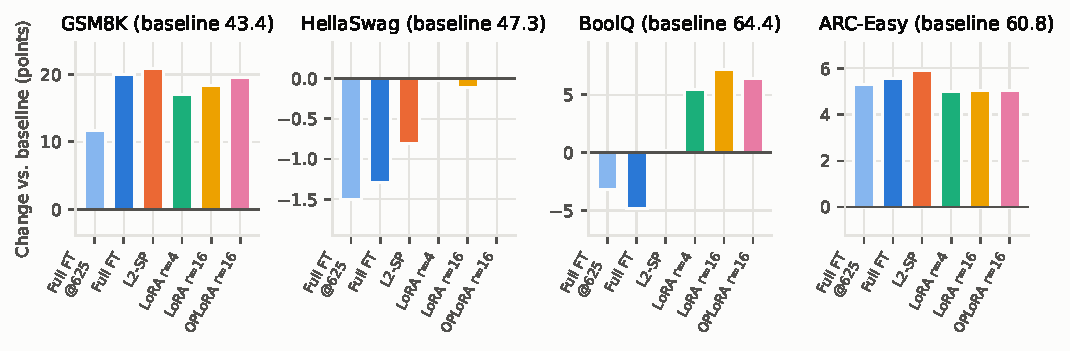
\includegraphics[width=0.9\linewidth]{figures/task1_benchmark_deltas.pdf}
\caption{Change from baseline (percentage points) per benchmark for the midpoint and the five final models.}
\label{fig:t1deltas}
\end{figure}

\begin{figure}[h]
\centering
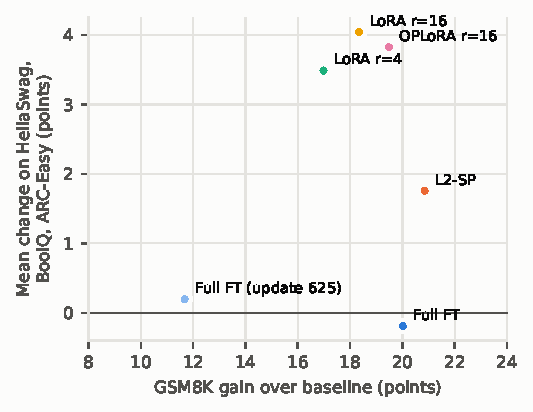
\includegraphics[width=0.45\linewidth]{figures/task1_adaptation_vs_retention.pdf}
\caption{GSM8K gain against the mean change on HellaSwag, BoolQ and ARC-Easy. Adapters sit high (retention gain) at
slightly lower adaptation; Full FT sits lowest.}
\label{fig:t1tradeoff}
\end{figure}

\begin{table}[h]
\caption{Weight-space and activation diagnostics on \texttt{down\_proj}. $\eta=\|\Delta W\|_F/\|W_0\|_F$; activation
ratio is mean $R(z)$ on math prompts over non-math prompts.}
\label{tab:t1diag}
\centering
\small
\begin{tabular}{lrrrrrrrrr}
\toprule
 & \multicolumn{3}{c}{$\rho_k$} & \multicolumn{3}{c}{$\eta$} & \multicolumn{3}{c}{Act.\ ratio} \\
Run & L0 & L13 & L27 & L0 & L13 & L27 & L0 & L13 & L27 \\
\midrule
Full FT (625) & 0.133 & 0.148 & 0.116 & 0.013 & 0.015 & 0.012 & 1.99 & 1.88 & 0.72 \\
Full FT & 0.133 & 0.148 & 0.115 & 0.014 & 0.016 & 0.013 & 1.98 & 1.85 & 0.71 \\
L2-SP & 0.133 & 0.150 & 0.107 & 0.011 & 0.014 & 0.008 & 2.01 & 1.71 & 0.74 \\
LoRA $r{=}4$ & 0.137 & 0.136 & 0.098 & 0.008 & 0.013 & 0.007 & 5.13 & 4.74 & 0.94 \\
LoRA $r{=}16$ & 0.129 & 0.153 & 0.107 & 0.014 & 0.019 & 0.011 & 2.97 & 3.01 & 0.93 \\
OPLoRA $r{=}16$ & 3.6e-08 & 2.9e-08 & 3.7e-08 & 0.014 & 0.019 & 0.009 & 3.95 & 3.22 & 1.01 \\
\bottomrule
\end{tabular}
\end{table}

\begin{table}[h]
\caption{Annotation of the fixed 42-response subset (first and last questions, three formats; six responses per
condition). Full labels, notes and excerpts are in \texttt{results/task1/qualitative\_annotation.json}. No response
contained inappropriate content.}
\label{tab:t1annot}
\centering
\small
\begin{tabular}{lrrrrr}
\toprule
Condition & Format followed & Coherent/relevant & Severe repetition & Math framing & Truncated \\
\midrule
Baseline & 5 & 3 & 0 & 0 & 0 \\
Full FT @625 & 2 & 0 & 3 & 3 & 3 \\
Full FT & 4 & 1 & 2 & 2 & 2 \\
L2-SP & 4 & 2 & 1 & 3 & 1 \\
LoRA $r{=}4$ & 5 & 3 & 0 & 0 & 0 \\
LoRA $r{=}16$ & 4 & 2 & 1 & 1 & 1 \\
OPLoRA $r{=}16$ & 5 & 3 & 0 & 2 & 0 \\
\bottomrule
\end{tabular}
\end{table}

\section{Additional Task 2 results}
\label{app:t2}

Calibration: mean text-embedding norm 0.799 and initial connector-output norm 15.89 (196 tokens) or 11.48 (49 tokens),
giving fixed scales 0.050 and 0.070. Training presented 72,000 examples (43,110 captions, 13,342 presence, 7,228 counting,
8,320 VQAv2, including replay); caption alignment made two full passes.

\begin{table}[h]
\caption{Task 2 accuracy (\%) by question type (196 tokens). The last row is the share of complementary-swap predictions
equal to the partner image's answer.}
\label{tab:t2types}
\centering
\small
\begin{tabular}{lrrrrr}
\toprule
Condition & Presence & Counting & Yes/no & Number & Other \\
\midrule
Correct image & 93.8 & 50.0 & 66.8 & 55.8 & 57.8 \\
Complementary swap & 6.2 & 26.6 & 42.8 & 17.9 & 17.9 \\
Mismatched & 46.9 & 15.6 & 50.7 & 27.5 & 9.2 \\
No image & 50.0 & 28.1 & 52.2 & 29.0 & 11.9 \\
\midrule
Swap follows partner answer & \multicolumn{2}{c}{71.9} & \multicolumn{3}{c}{58.3} \\
\bottomrule
\end{tabular}
\end{table}

\section{Additional Task 3 results}
\label{app:t3examples}

\begin{figure}[h]
\centering
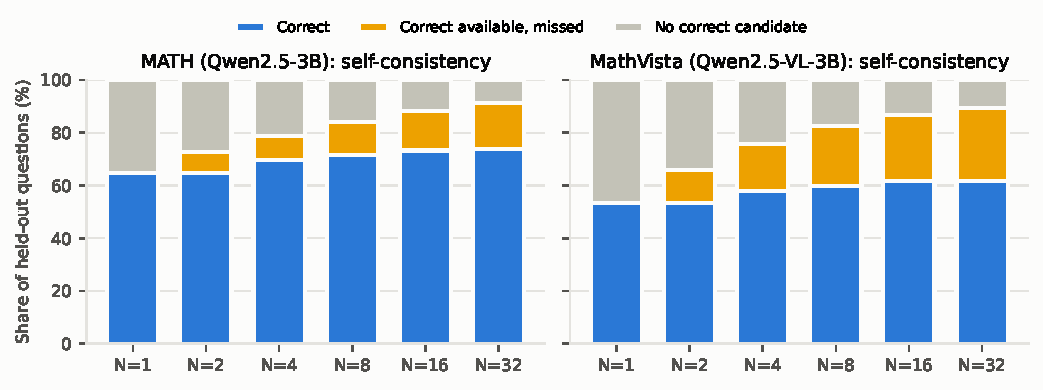
\includegraphics[width=0.9\linewidth]{figures/task3_failure_decomposition.pdf}
\caption{Self-consistency outcomes by budget: correct, correct candidate available but not selected, and no correct
candidate.}
\label{fig:t3decomp}
\end{figure}

\begin{figure}[h]
\centering
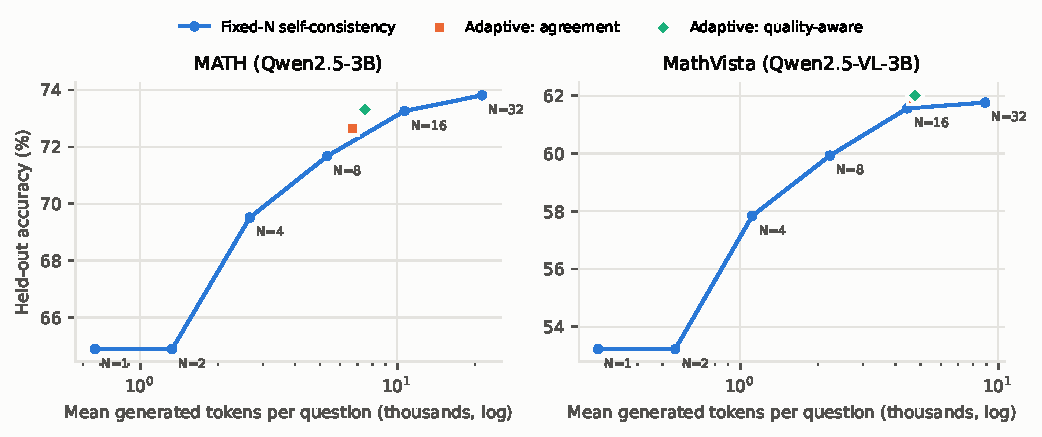
\includegraphics[width=0.9\linewidth]{figures/task3_accuracy_vs_cost.pdf}
\caption{Accuracy against mean generated tokens per question: fixed-$N$ self-consistency and the two adaptive policies
selected on development questions.}
\label{fig:t3cost}
\end{figure}

\begin{figure}[h]
\centering
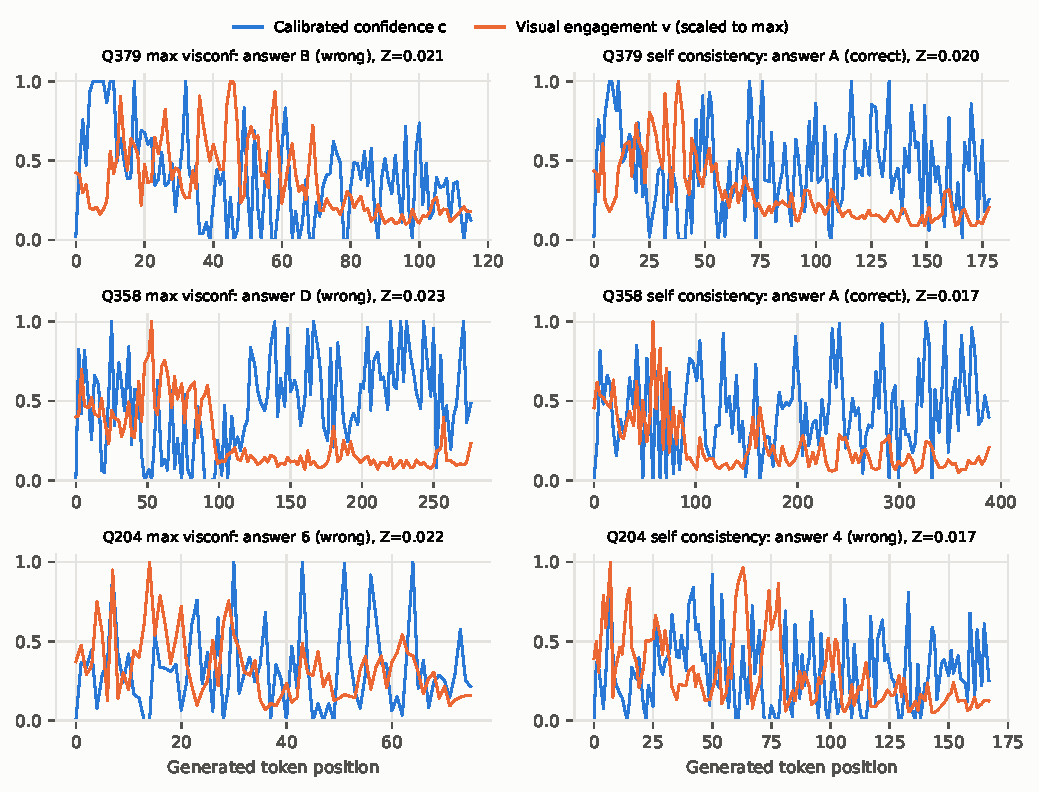
\includegraphics[width=0.9\linewidth]{figures/task3_trajectories.pdf}
\caption{Token-level calibrated confidence and visual engagement for fixed illustrative MathVista trajectories.
Selection rule: the first three held-out questions where max-VisConf and self-consistency disagree at $N{=}32$; left,
the top-VisConf rollout; right, the earliest rollout of the SC answer.}
\label{fig:t3traj}
\end{figure}

\textbf{Example cases} (selection rules in \texttt{task3/examples.py}; full records in \texttt{results/task3/examples/}).
\emph{Selection disagreement, MATH:} a question with gold answer 2 receives 16 votes for 0 and 15 for 2; SC returns 0,
self-certainty RWC returns 2. \emph{MathVista:} 11 votes for C against 10 for A (gold A); VisConf RWC selects A. In the
third MATH case both rules are wrong because the correct answer never appears. \emph{Premature stopping:} every
selected case stops at $n{=}4$ with 2 of 4 (MATH) or 3 of 4 (MathVista) votes, which the full pool reverses (for example
D with 13 of 32 votes against the early C). \emph{Revision:} the one wrong-to-correct case started from a 1,024-token
initial response that was cut off before its answer; the revision completed it (answer 216). In two other cases the
revision supplied an answer that was still wrong (1 for gold $-71$; $\sqrt{97.75}$ for gold 7).

\end{document}
